\documentclass[tikz]{standalone}
\usepackage{xcolor}
\usetikzlibrary{arrows,positioning,quotes,hobby,backgrounds,arrows.meta,bending,positioning,shapes,shapes.geometric}
\begin{document}
\pgfdeclarelayer{background}
\pgfsetlayers{background,main}
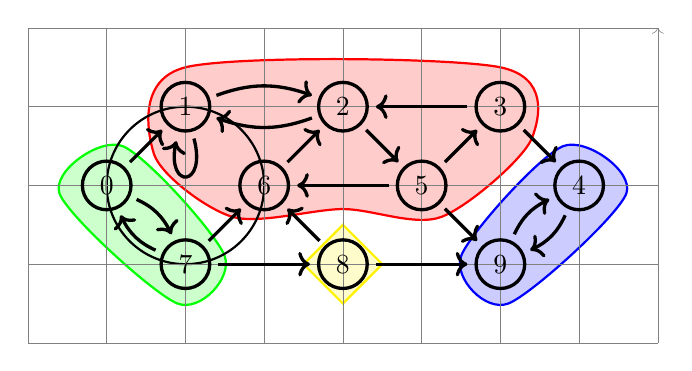
\begin{tikzpicture}
	[very thick,every circle node/.style={draw,outer sep=1.1mm}, every path/.style={->}]

\draw[thick] plot[smooth cycle,tension=1]
coordinates{(0,0)(1,1)(2,0)(1,-1)};

	\draw [help lines] (-1,-2) grid (7,2);
	\node[circle] (0) at (0,0) {0};
	\node[circle] (1) at (1,1) {1};
	\node[circle] (2) at (3,1) {2};
	\node[circle] (3) at (5,1) {3};
	\node[circle] (4) at (6,0) {4};
	\node[circle] (5) at (4,0) {5};
	\node[circle] (6) at (2,0) {6};
	\node[circle] (7) at (1,-1) {7};
	\node[circle] (8) at (3,-1) {8};
	\node[circle] (9) at (5,-1) {9};

	\path (0) edge (1);
	\path (0) edge[bend left=20] (7);
	\path (1) edge[loop below] (1);
	\path (1) edge[bend left=20] (2);
	\path (2) edge[bend left=20] (1);
	\path (2) edge (5);
	\path (3) edge (2);
	\path (3) edge (4);
	\path (4) edge[bend left=20] (9);
	\path (5) edge (3);
	\path (5) edge (6);
	\path (5) edge (9);
	\path (6) edge (2);
	\path (7) edge[bend left=20] (0);
	\path (7) edge (6);
	\path (7) edge (8);
	\path (8) edge (6);
	\path (8) edge (9);
	\path (9) edge[bend left=20] (4);

	\begin{pgfonlayer}{background}
		\draw[thick, red, fill=red!20!white] plot [smooth cycle] coordinates{(0.6,0.4)(1,1.5)(5,1.5)(5.4,0.6)(4.25,-.4)(3,-.3)(1.6,-.4)};
		\draw[thick, green, fill=green!20!white] plot [smooth cycle] coordinates{(0.2,0.5)(1.5,-0.9)(.9,-1.5)(-.6,-.1)};
		\draw[thick, blue, fill=blue!20!white] plot [smooth cycle] coordinates{(5.8,0.5)(4.5,-0.9)(5.1,-1.5)(6.6,-.1)};
        \draw[thick, yellow, fill=yellow!20!white,tension=0] plot [smooth cycle] coordinates{(3,-0.5)(3.5,-1)(3,-1.5)(2.5,-1)};
	\end{pgfonlayer}
\end{tikzpicture}

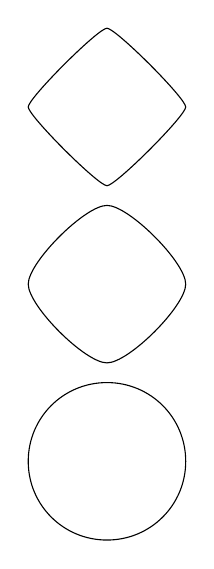
\begin{tikzpicture}[smooth cycle]
\draw plot[tension=0.2]
coordinates{(0,0) (1,1) (2,0) (1,-1)};
\draw[yshift=-2.25cm] plot[tension=0.5]
coordinates{(0,0) (1,1) (2,0) (1,-1)};
\draw[yshift=-4.5cm] plot[tension=1]
coordinates{(0,0) (1,1) (2,0) (1,-1)};
\end{tikzpicture}
\end{document}
